\documentclass{article}

\usepackage[utf8]{inputenc}
\usepackage[T1]{fontenc}
\usepackage[francais]{babel}
\usepackage{url}
\usepackage{color}
\usepackage{verbatim}
\usepackage{amsmath,amssymb,amsfonts}
\usepackage{graphicx}
\usepackage[french]{algorithm2e}
\usepackage{geometry}
\usepackage{enumitem}
\usepackage{listings}
\usepackage{listingsutf8}
\usepackage{caption}
\captionsetup[figure]{slc=on}
\frenchbsetup{StandardLists=true}
\lstset{language=Java}
\lstset{
	breaklines=true, 
	showspaces=false, 
	keepspaces=true, 
	numbers=left, 
	frame=single, 
	keywordstyle=\color{blue},
	basicstyle=\ttfamily\small,
	commentstyle=\color{green}
}
\geometry{hmargin=2.5cm, vmargin=2.5cm}

\title{Conception des Systèmes d'Exploitation\\Rapport sur les performances de l'allocateur mémoire}
\author{Line \bsc{POUVARET}, Mickaël \bsc{TURNEL}}
\date{2015-2016}

\begin{document}
\maketitle
\section{Présentation de la/les métriques évaluée(s)}
Nous avons choisi d'effectuer des mesures sur l'étalement du programme dans la mémoire (donc jusqu'à la dernière zone libre de la mémoire) et le montant de mémoire utilisé par le programme (cumul des tailles des blocs occupés de mémoire).

\section{Description de l'expérience menée}
Pour ce faire :
\begin{itemize}
\item A chaque allocation, on récupère la taille totale demandée, la taille cumulée des zones occupées et l'étendue de la mémoire.

\item A chaque libération, on récupère la taille cumulée des zones occupées et l'étendue de la mémoire.
\end{itemize}

Pour une simplification des mesures, les tailles prises correspondent aux données + leurs méta-données. Ce qui donne la taille réelle de la mémoire utilisé par l'allocateur et non pas seulement la taille de la mémoire que l'utilisateur utilise.\\

Nous avons repris notre allocateur du TP2 que nous n'avons pas modifié car les extensions demandées avaient déjà été faites (cf README.pdf pour tout détails). Nous nous sommes servis du Makefile du TP2 qui permet d'utiliser notre allocateur lors de l'exécution d'un programme.\\

Ainsi nous avons effectué les tests de notre allocateur sur plusieurs programmes: \textbf{ls}, \textbf{grep} et \textbf{gcc -C test.c} (test.c est un programme d'un de notre ancien TP sur la synchronisation).\\

Malheureusement, le test avec grep nous a pas paru pertinent puisqu'on observait très peu de fragmentation.

\section{Résultats obtenus}

\newpage
\subsection{Avec la stratégie First Fit}

\begin{figure}[h]
	\centering
	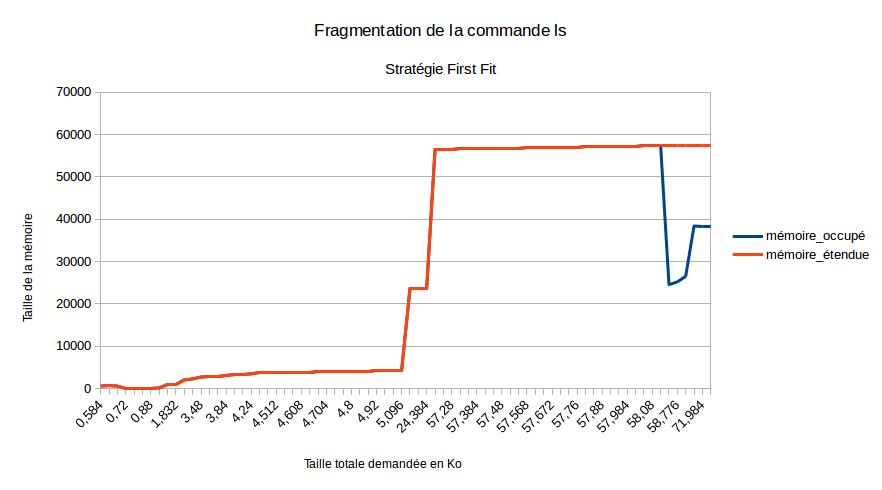
\includegraphics[width=14cm]{ls_firstfit.jpg}
	\caption{Programme ls avec First Fit}
\end{figure}

\begin{figure}[h]
	\centering
	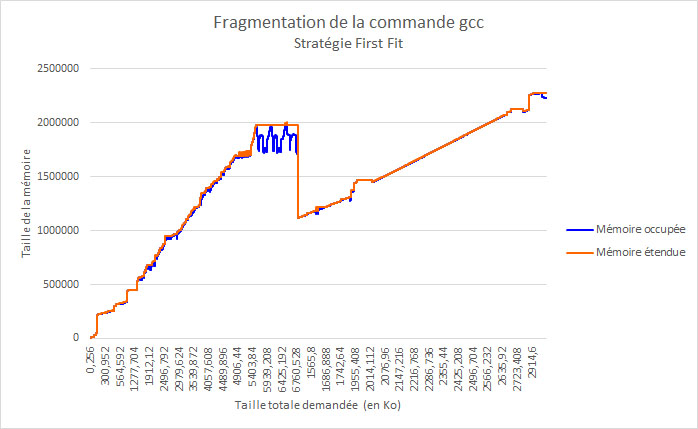
\includegraphics[width=12cm]{gcc_firstfit.jpg}
	\caption{Programme gcc avec First Fit}
\end{figure}

\newpage
\subsection{Avec la stratégie Best Fit}
\begin{figure}[h]
	\centering
	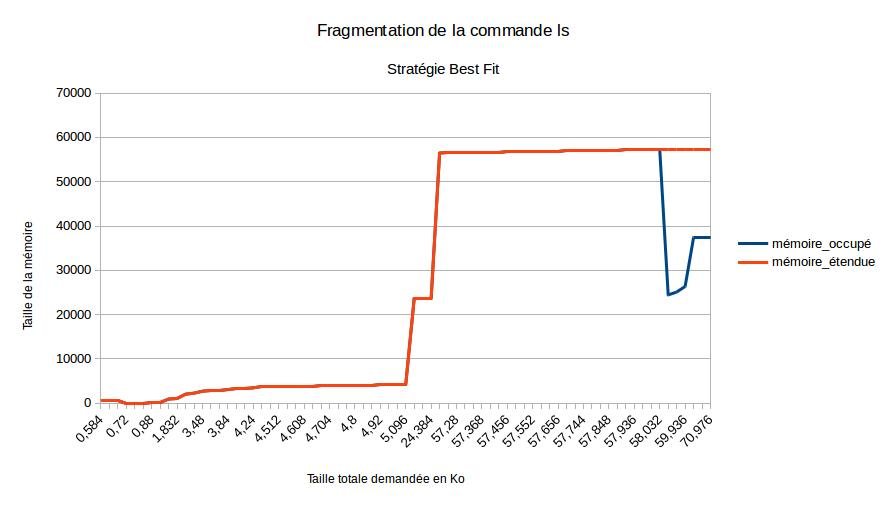
\includegraphics[width=14cm]{ls_bestfit.jpg}
	\caption{Programme ls avec Best Fit}
\end{figure}

\begin{figure}[h]
	\centering
	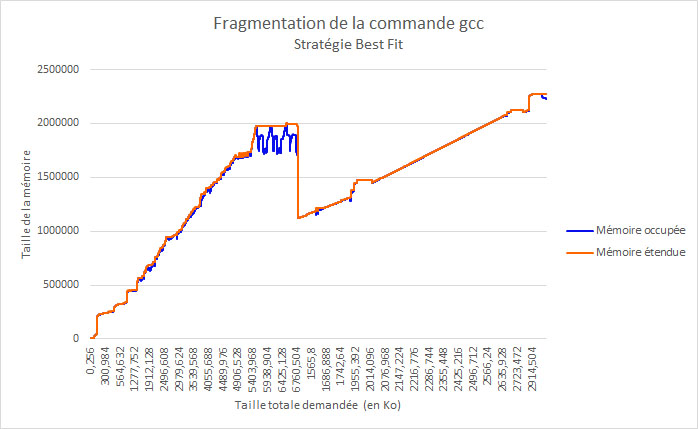
\includegraphics[width=12cm]{gcc_bestfit.jpg}
	\caption{Programme gcc avec Best Fit}
\end{figure}

\newpage
\subsection{Avec la stratégie Worst Fit}
\begin{figure}[h]
	\centering
	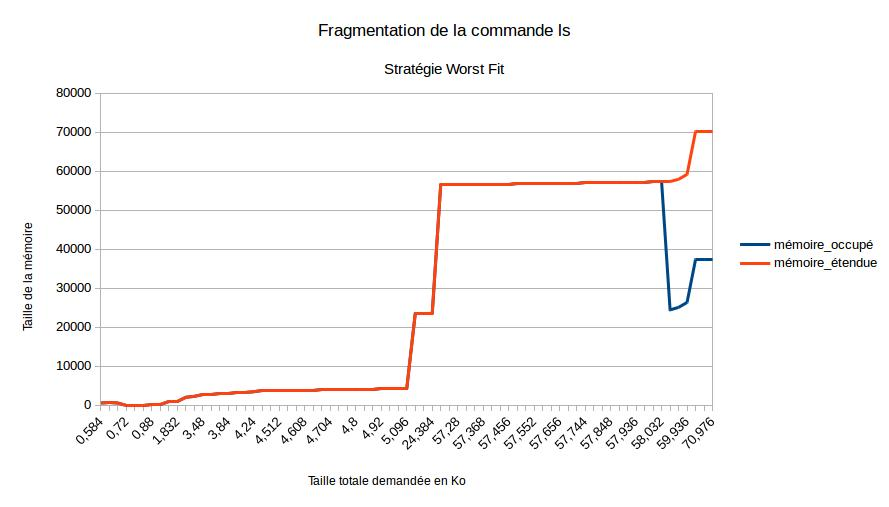
\includegraphics[width=14cm]{ls_worstfit.jpg}
	\caption{Programme ls avec Worst Fit}
\end{figure}

\begin{figure}[h]
	\centering
	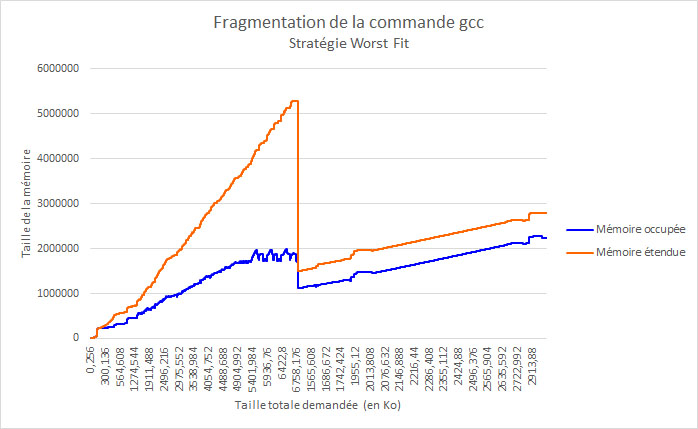
\includegraphics[width=12cm]{gcc_worstfit.jpg}
	\caption{Programme gcc avec Worst Fit}
\end{figure}

\newpage
\section{Conclusions}

\subsection{Programme ls}

On remarque (cf Fig. 1, 3 et 5) que la fragmentation a lieu sur la fin de l'appel de ls.\\
Le programme libère beaucoup de mémoire à $\sim$58 Ko, plus de la moitié, mais l'étendue ne bouge pas.\\

Puis d'autres allocation remonte la mémoire occupée sans pour autant accroître l'étendue de la mémoire utilisé sur les figures 1 et 3. Ceci est du à la stratégie qui va se servir des zones libres formées en plein "milieu" pour faire nos allocations. Cependant sur la figure 5 lors de ces dernières allocations l'étendue augmente elle aussi, ce qui est normal car la stratégie ici est le Worst Fit ce qui implique que le résidu formé par l'allocation au "milieu" de notre étendu n'était pas maximal d'où l'augmentation de celle-ci.

\subsection{Programme gcc}

Sur les figures 2 et 4, on remarque que le programme demande vite beaucoup de mémoire et arrivé à 2000000 (2 Mo) on peut apercevoir de la fragmentation. Puis $\sim$1 Mo de données est libérée sans créé de fragmentation on en déduit ici que les blocs occupés libérés étaient ceux se trouvant le plus "loin" et qui provoquaient une étendue plus importante dans la mémoire.\\
Enfin d'autres allocations sont faites sans créé de fragmentation.\\

Cependant la stratégie Worst Fit sur le programme \textit{gcc} n'a pas le même impact (Fig. 6). En effet, la mémoire est très fragmentée. Le programme utilisait au maximum $\sim$2.25 Mo de mémoire alors qu'ici le plus gros pic en mémoire est de plus de 5 Mo, plus du double. Mais à partir de $\sim$6.7 Mo de taille totale demandé, la fragmentation diminue fortement pour revenir à un état plus cohérent.\\
Enfin, à partir de ce point la fragmentation est toujours présente mais reste constante.\\

La stratégie Worst Fit est donc fortement déconseillé sur notre allocateur avec gcc.

\subsection{Conclusion}

On remarque tout d'abords que ce soit pour le programme \textbf{ls} ou le programme \textbf{gcc}, les versions First Fit et Best Fit n'ont presque aucune différence.\\
Alors qu'avec Worst Fit on voit tout de suite que la fragmentation est différente.\\

La version Worst Fit provoque plus de fragmentation ce qui est "logique" car on va chercher à utiliser la zone libre générant le plus gros résidu lors d'une allocation. Donc notre allocateur va avoir tendance à beaucoup plus étendre la mémoire du programme.\\

La stratégie influe donc naturellement sur la fragmentation de l'allocateur et le choix de celle ci dépendra des programmes utilisés par l'allocateur.

\end{document}